\subsection{实验目的-了解 iptables 中的表和链}
了解 iptables 中的表和链.
%
\subsection{实验原理}
\begin{itemize}
  \item Netfilter/iptables 是表(tables)的容器,iptables 包含 4 个表,分别是 filter、nat、mangel 和 raw。
  \item iptables 的表(tables)是链(chains)的容器,iptables 包含 5 个链,分别
    是 INPUT、OUTPUT、FORWARD、PREROUTING 和 POSTROUTING。
\end{itemize}
%
\subsection{实验原理}
\subsubsection{iptables 的表(tables)和链(chains)}
虽然 iptables 包含 4 个表,但是因为表 raw 在实际中很少或者基本上用不
到,所以默认情况下,iptables 根据功能和表的定义划分包含 3 个表:filter、
nat 和 mangel,其中,比较常用到的是 filter 和 nat。每个表又包含不同的操
作链(chains)。

下面的表格展示了表和链的对应关系,其中,1 表示有,0 则表示没有。
注意,所有链名必须大写。
\begin{table}[H]
  \begin{center}
    \begin{tabular}[c]{llllll}
      \hline
      表(tables)/链(chains) & INPUT & FORWARD & OUTPUT & PREROUTING & POSTROUTING \\
      \hline
      filter & 1 & 1 & 1 & 0 & 0 \\
      nat & 0 & 0 & 1 & 1 & 1 \\
      mangel & 1 & 1 & 1 & 1 & 1 \\
      \hline
    \end{tabular}
  \end{center}
\end{table}

下图展示了 filter 表和链 INPUT、FORWARD 和 OUTPUT 之间的对应关系。
\begin{figure}[H]
  \begin{center}
    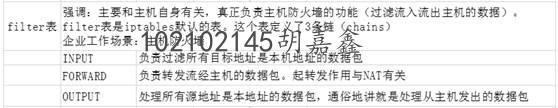
\includegraphics[width=0.40\textwidth]{2_3_1.jpeg}
  \end{center}
\end{figure}

下图展示了 nat 表和链 OUTPUT、PREROUTING 和 POSTROUTING 之间的对应关系。
\begin{figure}[H]
  \begin{center}
    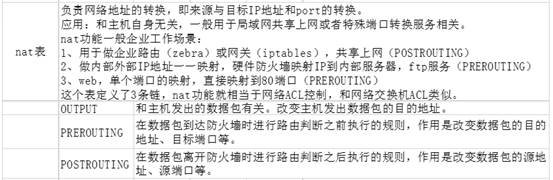
\includegraphics[width=0.40\textwidth]{2_3_2.jpeg}
  \end{center}
\end{figure}

Mangel 表主要负责修改数据包特殊的路由标记,如 TTL、TOS、MARK 等。由
于 mangel 表与特殊标记相关,一般情况下用不到这个表,这里就不做详细介绍
了。
%
\subsubsection{iptables 表和链工作的流程图}
下图清晰的描绘了 netfilter 对包的处理流程。
\begin{figure}[H]
  \begin{center}
    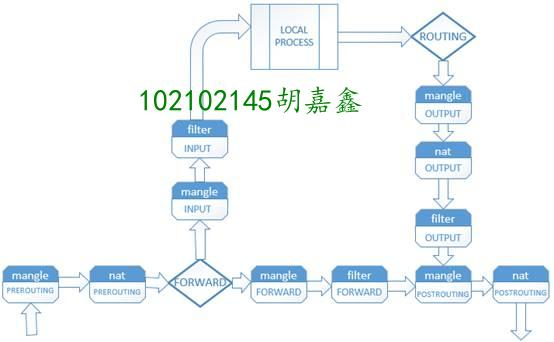
\includegraphics[width=0.40\textwidth]{2_3_3.jpeg}
  \end{center}
\end{figure}

为了更好的学习 iptables,可以将上图进行简化。
\begin{figure}[H]
  \begin{center}
    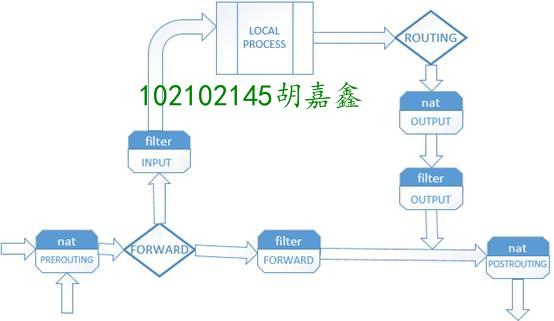
\includegraphics[width=0.40\textwidth]{2_3_4.jpeg}
  \end{center}
\end{figure}

上图可分为两个流程,上面的流程主要是 NAT 功能,在企业中常用于局域网
共享、将外部 IP 和端口映射为内部 IP 和端口等。下面的流程主要是 FILTER 功
能,即防火墙功能,企业中主要的应用是服务器防火墙。
